\subsection{Фундаментальная система решений и общее решение нормальной линейной однородной
системы уравнений}

Рассмотрим систему вида 
\begin{equation}
    \label{eq7:SLDE}
    \dot{\vec{x}} = A \vec{x} + \vec{f},
\end{equation} 
где $A = || a^i_j||$, $i,\,j = \overline{1, n}$ - матрица системы, 
причём $a^i_j$ - числа; 
$ \vec{f}(t) = 
  \begin{Vmatrix}
    f^1(t) \\
    \cdots    \\
    f^n(t)
  \end{Vmatrix}$ - вектор-столбец неоднородной системы;
$\vec{x}(t) = 
\begin{Vmatrix}
  x^1(t) \\
  \cdots    \\
  x^n(t)
\end{Vmatrix}$ - вектор-столбец искомых функций.  


Наряду с вышеприведённой записью также будем рассматривать запись вида: 
$$\frac{dx^i}{dt} = \sum\limits^n_{j=1}a^i_j x^j(t) + f^i, ~i = \overline{1, n}$$

Основная идея решения систем дифференциальных уравнений вида \eqref{eq7:SLDE}, 
состоит в том, что матрица системы рассматривается как матрица линейного преобразования 
линейного пространства $\vec{\mathbb{R}}^n$ (пространство, присоединнёное к аффинному 
$\mathbb{R}^n$), заданная в исходном базисе. 

Пусть $S = \begin{Vmatrix} \sigma_j^i \end{Vmatrix}$, $i,\,j = \overline{1, n}$ - матрица перехода от исходного базиса $\begin{Vmatrix} \vec{e_1}, ..., \vec{e_n} \end{Vmatrix}$ к базису. 
Эти соотношения связаны выражением $\begin{Vmatrix} \vec{e_1}, ..., \vec{e_n} \end{Vmatrix} = \begin{Vmatrix} \vec{e'_1}, ..., \vec{e'_n} \end{Vmatrix} \cdot S $ 
или $\vec{e'_i} = \sum\limits_{k = 1}^n \sigma_i^k \vec{e_k}$, а координаты векторов в новом и старом базисе связаны формулой $\vec{x} = S \vec{x'}$ или $x^i = \sum\limits_{m = 1}^n \sigma_m^i {x'}^m$.

Матрица перехода $S$ обратима, поэтому $\exists S^{-1} = \begin{Vmatrix} \tau_j^i \end{Vmatrix}$, $i,\,j = \overline{1, n}$, причём $SS^{-1} = S^{-1}S = E$, 
т.е. $\sum \limits_{k = 1}^n \tau_k^i \sigma_j^k = \delta_j^i$. Тогда $\vec{x'} = S^{-1}\vec{x}$.
Преобразуем исходную систему, умножив её справа на $S^{-1}$.

\[ S^{-1} \frac{d\vec{x}}{dt} = \frac{d}{dt} (S^{-1}\vec{x}) = S^{-1}A\vec{x} + S^{-1}\vec{f}\]

Подставив $\vec x = S \vec{\bar{x}}$, получим $\frac{d\vec{\bar{x}}}{dt} = \bar{A} \vec{x} + \vec{\bar{f}}$, где $\vec{\bar{f}}(t) = S^{-1}\vec{f}(t)$, 
а $\bar{A} = S^{-1}AS$ является матрицей преобразования $A$ в новом базисе. Уравнение имеет \textbf{ковариантный вид}, поэтому задачи свелись к нахождению базиса, в котором система имела бы наиболее простой вид.

Пусть $A$ - матрица системы \eqref{eq7:SLDE} является матрицей линейного преобразования линейного пространства $\vec{\mathbb{R}}^n$, 
т.е. $\forall \vec{x} \in \vec{\mathbb{R}}^n \mapsto A\vec{x} = \vec{y} \in \vec{\mathbb{R}}^n$, тогда $A = \begin{Vmatrix} A\vec{e_1}, ..., A\vec{e_n} \end{Vmatrix}$, 
т.е столбцы матрицы $A$ являются компонентами образов базисных векторов.


\begin{definition}
    Подпространство $L \subset \vec{\mathbb{R}}^n$ называется \textbf{инвариантным} подпространством относительно преобразования $A$, если $\forall \vec{x} \in L \mapsto A \vec{x} \in L$.
\end{definition}

Пусть $\vec{e}_1, ..., \vec{e}_s, \vec{e}_{s+1}, ..., \vec{e}_n$ - базис в $\vec{\mathbb{R}}^n$, а $\vec{e}_1, ..., \vec{e}_s$ - базис в $L$. \\
Тогда $\forall i = \overline{1, s} \mapsto A\vec{e_i} = \sum\limits_{k=1}^s \gamma_i^k \vec{e_k}$ и матрица $A$ в этом базисе будет иметь вид:

\[ A = \begin{Vmatrix} A_1 & A_2 \\ O & A_3 \end{Vmatrix}, \text{ где } A_1 = \begin{Vmatrix} \gamma_1^1 & \cdots & \gamma_s^1 \\ \vdots & & \vdots \\ \gamma_1^s &\cdots & \gamma_s^s\ \end{Vmatrix}, ~O \text{ - нулевая матрица размером } (n - s) \times s. \]

Если $\vec{\mathbb{R}}^n = L^1 \oplus ... \oplus L^k$ и $L^i, ~i = \overline{1, k}$ - инвариантные подпространства, то в базисе, который является базисом-объединения всех базисотв инваритных подпространств, прямая сумма которых равна $\vec{\mathbb{R}}^n$, матрица будет иметь вид:
\[A = \begin{Vmatrix} A_1 & O & \cdots & O \\ O & A_2 & \cdots & O \\ \cdots & \cdots & \cdots & \cdots \\ O & O &\cdots & A_k \end{Vmatrix} \] 

$A_i, ~i = \overline{1, k}$ - квадратная матрица размерами $l_i < n$, которая является сужением матрицы преобразования $A$ на инвариантное подпространство $L_i$

В таком случае искомую вектор-функцию можно переписать в виде: 
\[ \vec{x}(t) = \begin{Vmatrix} x^1 \\ \cdots \\ x^{l_1} \\ \cdots \\ x^{l_1 + ... + l_{i-1} + 1} \\ x^{l_1 + ... + l_{i}} \\ \cdots \\ x^{l_1 + .. l_k + 1} \\ \cdots \\ x^n \end{Vmatrix}\]

\[\text{Обозначим через } X_i = \begin{Vmatrix} x^{l_1 + ... + l_{i-1} + 1} \\ \cdots \\ x^{l_1 + .. + l_{i-1} + l_{i}}\end{Vmatrix} \]

Тогда система \eqref{eq7:SLDE} распадается на $k$ систем, порядок которых $l_i < n$: \\
$\dot{\vec{X_i}} = A_i \vec{X_i} + \vec{f_i}(t), ~i =\overline{1, k}$

Для приведения матрицы линейного преобразования к клеточно-диагональному виду нужно найти собственные векторы линейного преобразования. 
Вектор $\vec{x} \neq 0$ называется собственным вектором линейного преобразования, матрица которого равна $A$, если $A\vec{x} = \lambda \vec{x}$. 
Пусть $A = \begin{Vmatrix} a_j^i \end{Vmatrix}, ~i,\,j = \overline{1, n}$, а $\begin{Vmatrix} x^1 \\ \cdots \\ x^n \end{Vmatrix}$ - компоненты собственного вектора.
Тогда компоненты собственного вектора должны удовлетворять системе однородных линенейных уравнений вида $|| A - \lambda E|| \vec{x} = 0$. 
Чтобы эта система имела ненулевое решение необходимо, чтобы $\det || A - \lambda E|| = P_n(\lambda) = (-1)^n \lambda^n + (-1)^{n-1} \Tr A + ... + \det A = 0$. \\
$P_n(\lambda)$ - характерестический многочлен матрицы $A$. 

\subsubsection*{Случай простых корней характеристического многочлена}
Рассмотрим однорудную систему с постоянными коэффициентами \begin{equation}
  \dot{\vec{x}} = A \vec{x} \label{eq:ODN}
\end{equation}. Задача состоит в том, чтобы найти вектор функции $\vec{x}_1, \, \dots, \, \vec{x}_n$, которые будут образовывать ФСР нашей системы. 

\subsubsection*{Корни характеристического многочлена $\lambda_1, \dots, \lambda_n$ простые и действительные.}

Таким $\lambda_1, \dots, \lambda_n$ соответствуют собственные векторы $\vec{h}_1, \dots, \vec{h}_n$ ($A \vec{h}_i = \lambda_i \vec{h}_i$)
Можно показать, что собственные вектора, соответствующие разным собственным значениям линейно независимы, 
поэтому существует базис из собственных векторов $\vec{h}_1, \dots, \vec{h}_n$, в котором матрица $A$ имеет вид: 
$\bar{A} = \begin{Vmatrix} \lambda_1 & 0 & \ldots & \\ 0 & \lambda_2 & \ldots \\  \vdots& \vdots & \ddots &  0 \\ & & 0 & \lambda_n \end{Vmatrix}$ 
Тогда система \eqref{eq:ODN} будет иметь следующий вид: 
\[ \begin{cases}
    \cfrac{d \vec{x\,}^1}{dt} = \lambda_1 \vec{x \,}^1 \\
    \cdots \\
    \cfrac{d \vec{x \,}^n}{dt} = \lambda_n \vec{x \,}^n
\end{cases} \Longrightarrow \]

вектор-функции $\varphi_1 = \begin{Vmatrix*} 1 \\ 0 \\ \vdots \\ 0 \end{Vmatrix*} e^{\lambda_1 t}$, ..., 
$\varphi_n = \begin{Vmatrix*} 0 \\ 0 \\ \vdots \\ 1 \end{Vmatrix*} e^{\lambda_n t}$ 
образует ФСР этой системы, т.к. являются линейно независимыми решениями.
Матрица перехода в этом случае $S = \begin{Vmatrix*} \vec{h}_1,  ...,  \vec{h}_n \end{Vmatrix*}$. 
Тогда получим, что \begin{equation}
  \vec{x}_1 = \vec{h}_1 e^{\lambda_1 t}, ..., \vec{x}_n = \vec{h}_n e^{\lambda_n t} \label{eq7:FSR}
\end{equation} является ФСР \eqref{eq:ODN}, т.к. $\vec{x}_i, \,i= \overline{1, n}$ из \eqref{eq7:FSR} являются решениями \eqref{eq:ODN}, 
линейная независимость вектор-функций $\vec{x}_1, ..., \vec{x}_n$ следует из того, что вронскиан \eqref{eq7:FSR} при $t=0$ является $det S \neq 0$ (свойство 10 вронскиана).
Тогда любое решение \eqref{eq:ODN} представимо в виде
\begin{equation}
  \vec{x} = c_1 \vec{h}_1 e^{\lambda_1 t} + ... + c_n \vec{h}_n e^{\lambda_n t}
\end{equation}

Можно доказать, что $\vec{x}_1, ..., \vec{x}_n$ - ФСР иначе:
\begin{lemma}
  Система функций $e^{\lambda_1t}, ..., e^{\lambda_n t}$, где все $\lambda_i$ - разные, является линейно независимой.  
\end{lemma}
\begin{proof}
  Составим линейную комбинацию, равную нулю: $c_1 e^{\lambda_1 t} + ... + c_n e^{\lambda_n t} = 0$ - продифференцируем $(n-1)$ раз и 
  запишем получившуюся систему для поиска $c_1, ..., c_n$

  \[
  \begin{cases}
    c_1 e^{\lambda_1 t} + ... + c_n e^{\lambda_n t} = 0 \\
    \lambda_1 c_1 e^{\lambda_1 t} + ... + \lambda_n c_n e^{\lambda_n t} = 0 \\
    \cdots \\
    \lambda_1^{n-1} c_1 e^{\lambda_1 t} + ... + \lambda_n^{n-1} c_n e^{\lambda_n t} = 0
  \end{cases} 
  \]

Система является однородной, поэтому имеет тривиальное решение, но единственное ли оно? 

\[ \Delta = \begin{vmatrix*}
  e^{\lambda_1 t} & \cdots & e^{\lambda_n t} \\
  \lambda_1 e^{\lambda_1 t} & \cdots & \lambda_n e^{\lambda_n t} \\
  \vdots &  & \vdots \\ 
  \lambda_1^{n-1} e^{\lambda_1 t} & \cdots & \lambda_n^{n-1} e^{\lambda_n t} \\
\end{vmatrix*} = e^{\lambda_1 t + ... + \lambda_n t} \begin{vmatrix*}
  1 & \cdots & 1 \\
  \lambda_1  & \cdots & \lambda_n  \\
  \vdots &  & \vdots \\ 
  \lambda_1^{n-1}  & \cdots & \lambda_n^{n-1} \\
\end{vmatrix*} = e^{\lambda_1 t + ... + \lambda_n t} \prod \limits_{1 \leq j < i \geq n} (\lambda_i - \lambda_j) \neq 0
\]

Полученный определитель это определитель Вандермонда, который равен нулю только, если какая-то пара $\lambda_i, \lambda_j$ совпадёт. 
Значит определитель не равен нулю по условию $\Rightarrow$ система имеет только тривиальное решение по теореме Крамера $\Rightarrow$ система линейно независима.
\end{proof}

\begin{lemma}
Система $\vec{\varphi}_1 = \vec{h}_1 e^{\lambda_1 t}, ..., \vec{\varphi}_n = \vec{h}_n e^{\lambda_n t}$ является ФСР. 
\end{lemma}

\begin{proof}
  $\vec{\varphi}_i = \vec{h}_i e^{\lambda_i t}$ является решением по построению. Рассмотрим $W(t)$: $W(t) = \begin{vmatrix*} \vec{h}_1 e^{\lambda_1 t} \,...\, \vec{h}_n e^{\lambda_n t}\end{vmatrix*}$, 
  при $t = 0$: $W(0) = \begin{vmatrix*} \vec{h}_1 \, ... \, \vec{h}_n \end{vmatrix*} \neq 0$, т.к. собственные вектора линейно независимые. 
  Следовательно, по 10 свойству определителя Вронского система линейно независимая.
\end{proof}

Итак, общее решение системы \eqref{eq:ODN} записывается в виде: 

\begin{equation*}
  \boxed{\vec{x}^{\text{ об}}_0 = c_1 \vec{h}_1 e^{\lambda_1 t} + ... + c_n \vec{h}_n e^{\lambda_n t}}
\end{equation*}

\subsubsection*{Корни характеристического многочлена $\lambda_1, \dots, \lambda_n$ простые, но среди них есть комплексные.}
Пусть есть комплексные собственное число $\lambda_k = r_k + i \omega_k$ и ему соответствующий комплесный собственный вектор $\vec{h}_k + i \vec{d}_k $, 
где $\vec{h}_k$, $\vec{d}_k$ - действительные вектора. Так как характеристический многочлен это многочлен с действительными коэффициентами, 
то комплексгый корень идет вместе с комплексно ему сопряженным, т.е. $\bar{\lambda}_k = r_k - i \omega_k$ тоже является корнем характеристического многочлена. 

Взяв комплексное сопряжение над равенством $A (\vec{h}_k + i \vec{d}_k) = (r_k + i \omega_k)(\vec{h}_k + i \vec{d}_k)$:

\[ \overline{A (\vec{h}_k + i \vec{d}_k)} = A (\vec{h}_k - i \vec{d}_k) = \overline{(r_k + i \omega_k)(\vec{h}_k + i \vec{d}_k)} = (r_k - i \omega_k)(\vec{h}_k - i \vec{d}_k) \]
Т.е. $\vec{h}_k - i \vec{d}_k$ является собственным вектором для $\vec{\lambda_k} = r_k - i \omega_k$.

Аналогично случайно действительных простых корней система принимает вид: 

\[ \begin{cases}
  \cfrac{d \vec{x}_1}{dt} = \lambda_1 \vec{x}_1 \\ 
  \ldots \\
  \cfrac{d \vec{x}_k}{dt} = (r_k + i \omega_k)\vec{x}_k \\
  \cfrac{d \vec{x}_{k+1}}{dt} = (r_k - i \omega_k)\vec{x}_{k+1} \\
  \ldots \\
  \cfrac{d \vec{x}_n}{dt} = \lambda_n \vec{x}_n
\end{cases}\]

ФСР такой системы будет комплексной: $\begin{vmatrix*} 1 \\ 0 \\ 0 \\ \vdots \\ \vdots \\ 0 \\ 0 \end{vmatrix*} e^{\lambda_1 t}$; ...; 
$\begin{vmatrix*} 0 \\ \vdots \\ 0 \\ 1 \\ 0 \\ \vdots \\ 0 \end{vmatrix*} e^{r_k t} (cos \omega_k t + i sin \omega_k t)$; \\
$\begin{vmatrix*} 0 \\ \vdots \\ 0 \\ 0 \\ 1 \\ \vdots \\ 0 \end{vmatrix*} e^{r_k t} (cos \omega_k t - i sin \omega_k t)$; ...; 
$\begin{vmatrix*} 0 \\ 0 \\ 0 \\ \vdots \\ \vdots \\ 0 \\ 1 \end{vmatrix*} e^{\lambda_n t}$

Т.к. матрица перехода $S = \begin{Vmatrix*} \vec{h}_1, \ldots, \vec{h}_k + i \vec{d}_k, \vec{h}_k - i \vec{d}_k, \ldots, \vec{h}_n \end{Vmatrix*}$, 
то комплексная ФСР \eqref{eq:ODN} будет: $\vec{h}_1 e^{\lambda_1 t}$, ..., $(\vec{h}_k + i \vec{d}_k) e^{r_k t} (cos\omega_k t + i sin \omega_k t)$, 
$(\vec{h}_k - i \vec{d}_k) e^{r_k t} (cos\omega_k t - i sin \omega_k t)$, ..., $\vec{h}_n e^{\lambda_n t}$  

Рассмотрим систему функций, у которых первые $k-1$ функции являются функциями построенной выше системы. В качестве $k$-ой и $k+1$-ой функций возьмём:

\[
   \vec{q}_k = \frac{1}{2}((\vec{h}_k + i \vec{d}_k) e^{r_k t} (cos \omega_k t + i sin \omega_k t) + (\vec{h}_k - i \vec{d}_k) e^{r_k t} (cos \omega_k t - i sin \omega_k t)) = e^{r_k t} (\vec{h}_k cos \omega_k t - \vec{d}_k sin \omega_k t)
\]

\[
   \vec{q}_{k+1} = \frac{1}{2i}((\vec{h}_k + i \vec{d}_k) e^{r_k t} (cos \omega_k t + i sin \omega_k t) - (\vec{h}_k - i \vec{d}_k) e^{r_k t} (cos \omega_k t - i sin \omega_k t)) = e^{r_k t} (\vec{h}_k sin \omega_k t + \vec{d}_k cos \omega_k t)
\]

Остальные вектор-функции оставим прежними. Так построенная система будет линейно независимой, т.к. была получена линейными комбинациями линейно независимых вектор-функций. Каждая функция данной системы будет решением \eqref{eq:ODN} по построению и принципу суперпозиции $\Rightarrow$ полученная система является ФСР \eqref{eq:ODN} и содержит только действительные функции $\Rightarrow$ 

\begin{equation*}
  \boxed{\vec{x}^{\text{ об}}_0 = c_1 \vec{h}_1 e^{\lambda_1 t} + ...+ c_k e^{r_k t} (\vec{h}_k cos \omega_k t - \vec{d}_k sin \omega_k t) + c_{k+1} e^{r_k t} (\vec{h}_k sin \omega_k t + \vec{d}_k cos \omega_k t) + ... + c_n \vec{h}_n e^{\lambda_n t}}
\end{equation*}

\subsubsection*{Случай кратных корней характеристического многочлена}

В общем случае по основной теореме алгебры характеристический многочлен представляется в виде: 
$P_n (\lambda) = (-1)^n \lambda^n + (-1)^{n-1}\Tr A + ... + det A = (\lambda - \lambda_1)^{k_1} \cdot ... \cdot (\lambda - \lambda_m)^{k_m}$, 
где $\lambda_1, ..., \lambda_m$ являются собственными числами матрицы $A$, $k_i \geq 1$, $i = \overline{1, m}$. 
В таком случае количество собственных вектором может быть меньше размерности пространства, поэтому матрица может быть не диагонализируема.

\begin{definition}
  Множество $R_s = \ker (A - \lambda_s E)^{k_s}$, $s = \overline{1, m}$, где $\lambda_s$ - корень кратности $k_s$ характеристического многочлена, называется \textbf{корневым пространством}
\end{definition}

Одно из утверждений теоремы Жордана: $\vec{R}^n = R_1 \oplus ... \oplus R_m $ пространство раскладывается в прямую сумму корневых подпространств, а также $dim R_s = k_s$.
Следовательно, если выбрать базис, как объединение базисов корневых подпространств, то исходная система распадается на $m$ систем порядка $k_s$, $s = \overline{1, m}$, связывающих $k_s \leq n$ функций. Рассмотрим одну из таких систем.

Обозначим $\lambda_s = \bar{\lambda}$, $k_s = l$, перенумеруем и переобозначим искомые функции $x^{k_1 + ... + k_{s-1} + 1} = \bar{x}_1$, ..., $x^{k_1 + ... + k_{s - 1} + l} = \bar{x}^l$ 
Тогда имеем задачу: решить систему
\begin{equation}
  \dot{\vec{\bar{x}}} = \bar{A} \vec{\bar{x}}
\end{equation}

где $\bar{A}$ является сужением $A$ на подпространство $R_s = \ker (A - \bar{\lambda} E)^{l} = \ker B^l$, т.е. $\forall \vec{\bar{x}} \in R_s \mapsto B^l \vec{\bar{x}} = 0$ по определению ядра. 

Имеет место вложенность: $ 0 \subset \ker B \subset \ker B^2 \subset ... \subset \ker B^l$, 
т.к. $\forall \vec{\bar{x}}: B^{i-1}(\vec{\bar{x}}) = 0 \mapsto B^{i}(\vec{\bar{x}}) = B(B^{i-1}(\vec{\bar{x}})) = 0$

Обозначим $T_i = \ker B^i$, $i = \overline{1, k}$, где $k \leq l$

\begin{remark}
  Неравенство $k \leq l$ связано с тем, что может оказаться, что $\forall \vec{\bar{x}} \in R_s \mapsto B^k \vec{\bar{x}} = 0$ и строить $T_i$ невозможно
\end{remark}

Для $i = \overline{1, k}$ определим множество $\mathcal{V}^i = \{\vec{\bar{x}} \in \mathcal{V}^i: B^i \vec{\bar{x}} =0 , B^{i-1}\vec{\bar{x}} \neq 0 \}$.
Заметим, что $\mathcal{V}^1$ является по построению собственным подпространством $A$.

В силу определения $B^i$ и $\mathcal{V}^i$: $\mathcal{V}^i = \ker B^i \setminus \ker B^{i-1}$, $i = \overline{2, k}$. По построению $R_s = \mathcal{V}^1 \oplus ... \oplus \mathcal{V}^k$. Осталось выбрать базис в $\mathcal{V}^i$, $i = \overline{2, k}$. 

\begin{figure}[!h]
  \centering
  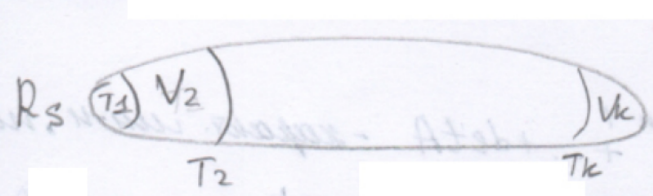
\includegraphics[width=0.5\linewidth]{"images/Issue7-1.png"}
  \caption[]{}
\end{figure}

\begin{theorem}
  Пусть $i > j$, тогда $\forall \vec{h}_i \in \mathcal{V}^i \, \exists \vec{h}_j \in \mathcal{V}^j: \vec{h}_j = B^{i-j}\vec{h}_i$.
\end{theorem}

\begin{proof}
  Построим такой $\vec{h}_j$ и покажем, что он лежит в $\mathcal{V}^j$.

  \[ B^j \vec{h}_j = B^j (B^{i-j}(h_i)) = (B^j B^{i-j} )(\vec{h}_i) = B^i \vec{h}_i = 0 \] 
  \[ B^{j-1} \vec{h}_j = B^{j-1} (B^{i-j}(h_i)) = (B^{j-1} B^{i-j} )(\vec{h}_i) = B^{i-1} \vec{h}_i \neq 0 \]
\end{proof}

Построение соответствующего базиса начинается с определения собственных векторов $A$, соответствующих числу $\bar{\lambda}$.
Для этого решается уравнение $(\bar{A} - \bar{\lambda} E) \vec{\bar{x}} = B  \vec{\bar{x}} = 0$.

Рассмотрим случай, когда имеется только один собственный вектор $\vec{e}$. В этом случае $k = l$ (наше подпространство будет представимо в виде 1 жордановой клетки). 
Вектор $\vec{e}$ образует базис в $\mathcal{V} = T_1$. Вектор $\vec{h}_1 \in \mathcal{V}^2$ найдём как решение $B \vec{h}_1 = \vec{e}$, по доказанной выше теореме такое уравнение имеет решение. 
Вектор $\vec{h}_1$ называется \textbf{присоединенным} к вектору $\vec{e}$. Вектора $\vec{e}$ и $\vec{h}_1$ образуют базис в $T_2$. 
Определим векторы $\vec{h}_i$, $i = \overline{2, l-1}$ из уравнений $B \vec{h_i} = \vec{h}_{i-1}$. Так построенные векторы $\vec{e}, \vec{h}_1, ..., \vec{h}_{l-1}$ образует базис в $R_s$. 
Этот базис называется жордановой цепью.

Запишем матрицу системы в этом базисе. Все построенные векторы находим из уравнений: 
$\bar{A}\vec{e} = \bar{\lambda} \vec{e}$, $\bar{A} \vec{h}_1 = \vec{e} + \bar{\lambda} \vec{h}_1$, ..., $\vec{A} \vec{h}_{l-1} = \vec{h}_{l-2} + \bar{\lambda} \vec{h}_{l-1}$

\[ \bar{A} = \begin{Vmatrix*} \bar{\lambda} & 1 & 0 & \cdots & \cdots \\
                              0 & \bar{\lambda} & 1 & 0 & \cdots     \\
                              \cdots & \cdots & \ddots & \cdots & \cdots \\
                              \cdots & \cdots & \cdots & \bar{\lambda} & 1 \\ 
                              \cdots & \cdots & \cdots & 0 & \bar{\lambda} 
             \end{Vmatrix*} \text{ - жорданова клетка размер $l$}
             \]

В таком базисе системе имеет вид:

\begin{equation}
 \begin{cases}
   \cfrac{d \bar{x}^{\,1}}{dt} = \bar{\lambda} \bar{x}^{\,1} + \bar{x}^{\,2} \\
   \ldots \\
   \cfrac{d \bar{x}^{\,n-1}}{dt} = \bar{\lambda} \bar{x}^{\,n-1} + \bar{x}^{\,n} \\
   \cfrac{d \bar{x}^{\,n}}{dt} = \bar{\lambda} \bar{x}^{\,n} \\
 \end{cases} 
\end{equation}

Замена: $\bar{x}^{\,i} = \bar{y}^{\,i} e^{\bar{\lambda} t}$, $i = \overline{1, l} \Rightarrow \dot{\vec{y}}^{\,i} e^{\bar{\lambda} t} + \bar{\lambda} \dot{\vec{y}}^{\,i} e^{\bar{\lambda} t} = \lambda \dot{\vec{y}}^{\,i} e^{\bar{\lambda} t} + \dot{\vec{y}}^{\,i+1} e^{\bar{\lambda} t} \Rightarrow$
Система преобразуется к виду:

\begin{equation}
  \begin{cases}
    \cfrac{d\bar{y}^{\,1}}{dt} = \bar{y}^{\,2} \\ 
    \cfrac{d\bar{y}^{\,2}}{dt} = \bar{y}^{\,3} \\
    \ldots \\
    \cfrac{d\bar{y}^{\,l-1}}{dt} = \bar{y}^{\,l} \\
    \cfrac{d\bar{y}^{\,l}}{dt} = 0
  \end{cases}
  \Rightarrow 
  \vec{y} = \begin{Vmatrix*} c_l \cfrac{t^{l-1}}{(l-1)!} + c_{l-1} \cfrac{t^{l-2}}{(l-2)!} + ... + c_2 \cfrac{t}{1!} + c_1 \\
                            \ldots \\
                            \ldots \\
                            c_l t + c_{l-1} \\
                            c_l \end{Vmatrix*} \Rightarrow  
\end{equation}

\begin{equation*}
  \Rightarrow \vec{\bar{x}} = \begin{Vmatrix*} c_l \cfrac{t^{l-1}}{(l-1)!} + c_{l-1} \cfrac{t^{l-2}}{(l-2)!} + ... + c_2 \cfrac{t}{1!} + c_1 \\
    \ldots \\
    \ldots \\
    c_l t + c_{l-1} \\
    c_l \end{Vmatrix*} \cdot e^{\bar{\lambda} t} 
\end{equation*}


Переходим к старому базису: 

\[ \vec{x}(t) = \begin{Vmatrix*}
  \vec{e}, \vec{h}_1, ..., \vec{h}_{l-1} 
\end{Vmatrix*} \cdot \begin{Vmatrix*} c_l \cfrac{t^{l-1}}{(l-1)!} + c_{l-1} \cfrac{t^{l-2}}{(l-2)!} + ... + c_2 \cfrac{t}{1!} + c_1 \\
\ldots \\
\ldots \\
c_l t + c_{l-1} \\
c_l \end{Vmatrix*} \cdot e^{\bar{\lambda} t} \Rightarrow \] 

\begin{multline}
 \vec{x}^{\text{ об}}_0 =  \vec{e} \left(c_1 + ... + c_l \cfrac{t^{l-1}}{(l-1)!} \right) e^{\bar{\lambda} t} + ... + \vec{h}_{l-1} c_l e^{\bar{\lambda} t} = \\ 
  = \boxed{c_1 \vec{e} e^{\bar{\lambda} t} + c_2 (\vec{e} t + \vec{h}_1) e^{\bar{\lambda} t} + ... + c_l \left[ \vec{e} \cfrac{t^{l-1}}{(l-1)!} + \vec{h}_1 \cfrac{t^{l-2}}{(l-2)!} + ... + \vec{h}_{l-1} \right]} 
\end{multline}

Полагая последовательно $c_1 = 1, c_2 = ... = c_n = 0$; ...; $c_1 = ... = c_{i-1} = c_{i+1} = ... = c_n = 0$, $c_i = 1$, $i = \overline{2, n}$ получим функции:

$\vec{\varphi}_1 = \vec{e} e^{\bar{\lambda} t}$, $\vec{\varphi}_1 = (\vec{e}t + \vec{h}_1) e^{\bar{\lambda} t}$, ..., $\vec{\varphi}_{l-1} = \left(\vec{e} \cfrac{t^{l-1}}{(l-1)!} + \vec{h}_1 \cfrac{t^{l-2}}{(l-2)!} + ... + \vec{h}_{l-1}\right) e^{\bar{\lambda} t}$. 
Они являются решениями по построению, $W(0) = \begin{vmatrix*} ||\vec{e}, ..., \vec{h}_{l-1} ||\end{vmatrix*} \neq 0 \Rightarrow \vec{\varphi}_1, ..., \vec{\varphi}_{l-1}$ - линейно независимы $\Rightarrow \vec{\varphi}_1, ..., \vec{\varphi}_{l-1}$ - ФСР. 

\subsection{Линейная неоднородная система уравнений в случае, когда неоднородность представлена векторным квазимногочленом}